
\section{Problem Formulation}
\subsection{The Electrode, Dielectric, and Droplet Problem}
\hspace{0em}\indent Consider a droplet situated on a dielectric layer, with electrodes charging the droplet/layer and altering the droplet curve's shape and contact angle, as shown in Figure \ref{fig:sketch electrode}.
    \begin{figure}[H]
        \centering
                \adjustbox{frame=.01pt,frame,margin=.01, color=mycolor}{
        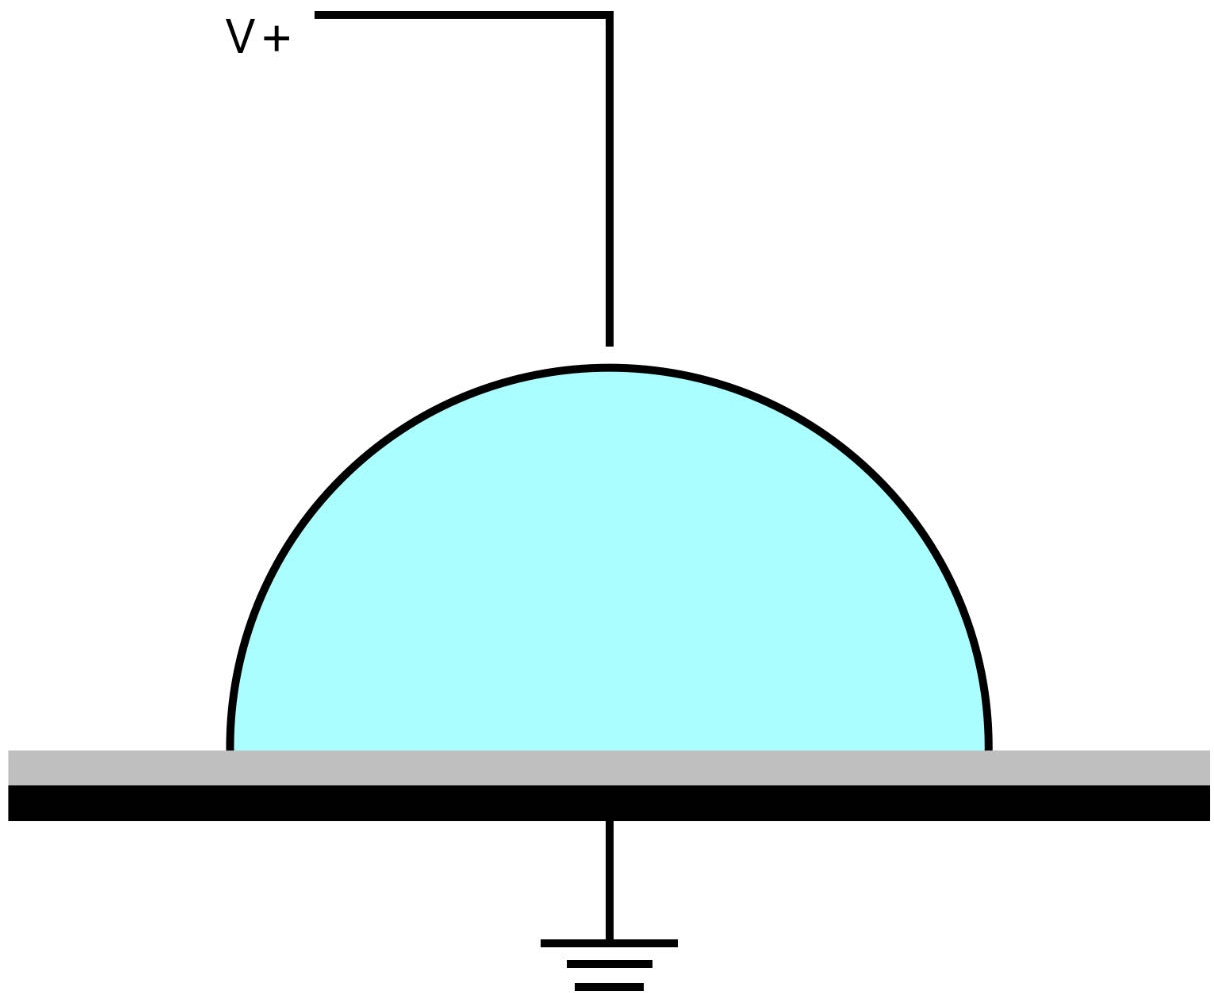
\includegraphics[width=0.7\linewidth]{Figs/sketch eletrode}}
        \caption{\small Sketch of the electrode, dielectric, and droplet problem. The $V_+$ electrode and grounded substrate create a voltage difference across the conducting droplet and layer.}
        \label{fig:sketch electrode}
    \end{figure}
Given the complexity of the functionalisation of the droplet's surface and other related issues, directly obtaining an analytical solution for its electric potential is difficult.

\subsection{The Simplification of the Problem}
\hspace{0em}\indent This study simplifies the problem in several stages. First, when observed from a distance, the droplet's shape degenerates into a thin film with negligible height, which we refer to as a ``slit". The dielectric layer is assumed to be semi-infinite in $-y$ and $\pm x$ directions relative to the slit. Second, the influence of the electrodes is simplified to a point charge, though its precise location and magnitude are not accurately depicted in the following figure, as these parameters may vary. Figure \ref{fig:slit} provides an approximate representation of the simplified Situation.

Additional characteristics of the simplified configuration include the surface charge on the boundary of the dielectric layer, the volume charge within the dielectric, and the voltage at infinity. The latter remains unknown and, at this stage, cannot be constrained in a manner that satisfies the uniqueness theorem (section \ref{thm:uniquenss}).

    \begin{figure}[H]
        \centering
        \adjustbox{frame=0.25pt,frame,margin=0.15,color=mycolor}{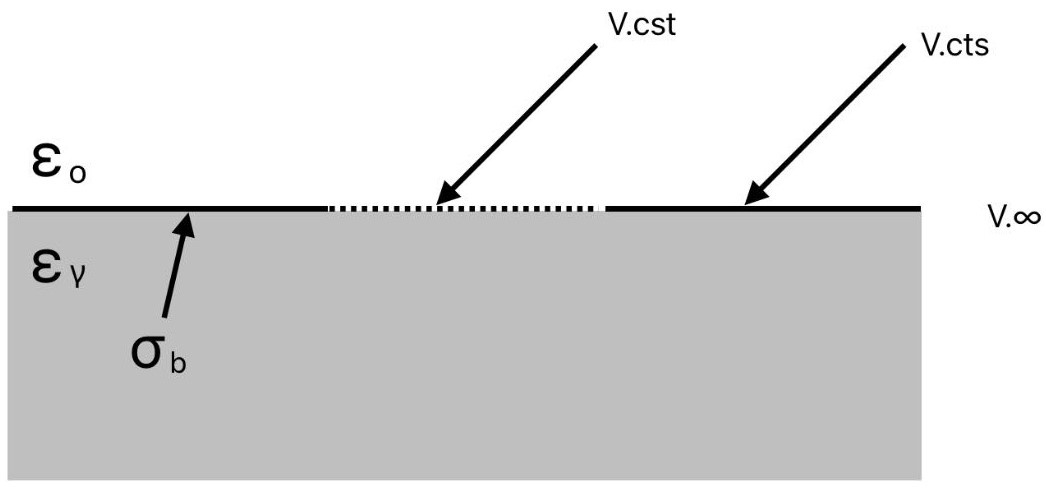
\includegraphics[width=.8\linewidth]{Figs/slit_e.jpg}}
        \caption{\small Thin droplet slit on the dielectric layer. The dashed line represents the slit, while the thick black lines indicate the boundaries of the dielectric and the air above. The shaded areas denote the dielectric, and the upper space of air is left blank. Additionally, $\epsilon_0$ and $\epsilon_{\gamma}$ are the electric permittivity of air and the dielectric, respectively. $\sigma_b$ is the surface charge density of the dielectric layer, with the surface charge density in the air is set to be zero. V.cst indicates the slit is itself an equipotential surface, V.cts means the voltage is continuous along the dielectric-air interface, and V.$\infty$ represents the far-field voltage, which is unknown.\\
        Lastly, it should be noted that we use a point charge to represent the electrodes, which is not shown in the sketch. This point charge is embedded somewhere in the dielectric and varies in magnitude due to the properties of the electrodes.}
        \label{fig:slit}
    \end{figure}
For other properties and coefficients not explicitly included in the sketch, we can now establish the boundary conditions:
\begin{itemize}
    \item All charges of the conductive droplet $\Omega$ are distributed along the boundary of the droplet.
    \vspace{-0.5em}
   \[\int_{\partial \mathcal{D}} \sigma_{\partial\Omega} \df l = Q_{\Omega}\vspace{-0.5em}
   \]
    \item There is an induced volume charge density $\rho$ at $\vec{r_0}$ in the dielectric, where the embedded point charge is located.
    \[
    \epsilon_0\nabla\cdot \mathbf{E}=\frac{q}{\epsilon_r}\delta(\vec{r}-\vec{r}_0)%\vspace{-1em}
    \]
    \item Except for the location of the embedded point charge, all induced charges in the dielectric $\mathcal{D}$ are distributed along the boundary of the dielectric and the air.
    \vspace{-.5em}
     \[\nabla\cdot \mathbf{E}=0\hspace{1em}\text{s.t. in }\mathcal{D}\setminus \{\partial \mathcal{D} \cup \vec{r}_0\}\vspace{-1em}\]
    \item The voltage of the conducting droplet is constant.
    \vspace{-0.5em}
    \[V(\Omega)=Constant\vspace{-1em}\]
    \item The voltage is continuous on the boundary $\partial \Omega$. The voltage $V^{(b)}$ represents that in the dielectric, and the air above has a voltage $V^{(a)}$ .
    \begin{equation}\label{eqn:v.cts}
\left.V^{(a)}\right|_{\partial\mathcal{D}^+}=\left.V^{(b)}\right|_{\partial\mathcal{D}^-}        
    \end{equation}
\end{itemize}
\vspace{-.5em}
\hspace{0em}\indent Yet some uncertain properties at this stage include:
\begin{itemize}
    \item There may be induced charges at the boundary $\partial\mathcal{D}$, caused by the presence of free charge(the point charge). let $\l^o$ be a small closed loop across the boundary $\partial\mathcal{D}$; Gauss's Law states that 
    \[\oint_{l^o} -\epsilon \nabla V\cdot\hat{n}\df l = \pi r^2\sigma_b\]
    or in terms of $\vec{E}$, since the boundary lies along the $x$-axis, only the $y$ component of $\vec{E}$ contributes:
    \begin{equation}\label{eqn:gauss}
    \epsilon_0 E^{(a)}_y-\epsilon_\gamma E^{(b)}_y=\sigma_b   
    \end{equation}
    
    However, charge distributions with no induced charge on the boundary between the dielectric and the space above do exist, as a later case shows.
    
    \item We are generally uncertain about the exact behaviour at infinity.  Besides the far-field voltage of a point charge, the voltage at infinity does not necessarily decrease, the semi-infinite dielectric may contribute.

    \item The equipotentials around the slit are unknown, as are those around the two cusps. Additionally, the induced charge of the slit mixes with that of the dielectric at the slit's lower boundary line\(\partial\Omega \cap \partial\mathcal{D}\).
\end{itemize}

although the droplet's height is ignored, the electric potential of the simplified problem remains challenging due to the boundary conditions.

\subsection{Apply the Joukowski Transformation}\label{cpt:jkw}

\hspace{0em}\indent The Joukowski transformation maps the slit to a disc. If we can determine an appropriate electric potential for the embedded disc, dielectric, and point charge scenario, we can use the inverse map to address the cusps. However, this approach introduces a new challenge due to the asymmetric dielectric geometry relative to the y-axis, as outlined in Figure \ref{fig: maped disc}.

\begin{figure}[H]
    \centering
    \adjustbox{frame=0.25pt,frame,margin=0.15,color=mycolor}{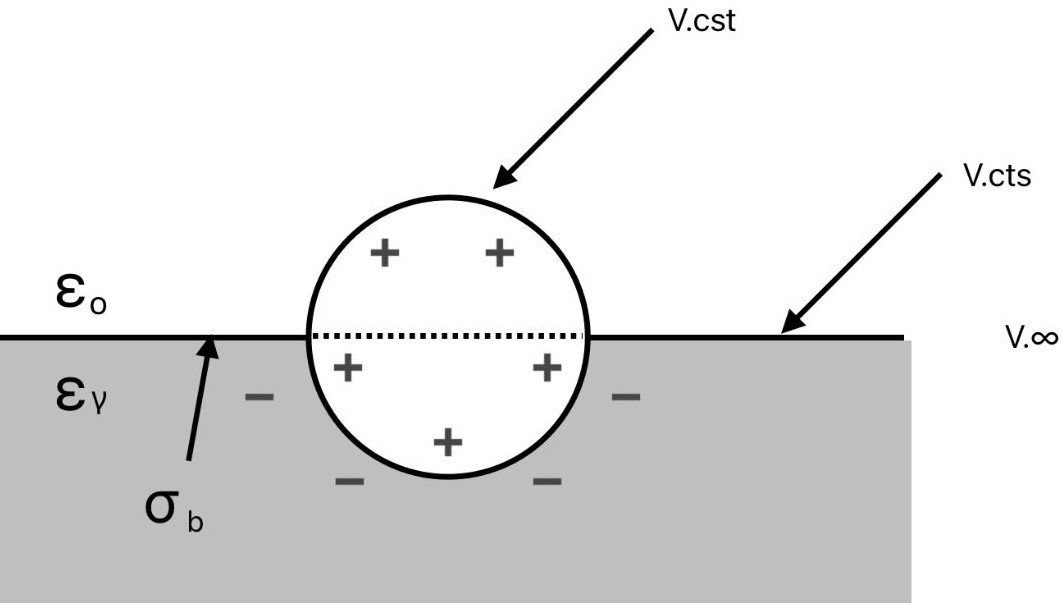
\includegraphics[width=.8\linewidth]{Figs/disk.jpg}}
    \caption{\small The problem corresponds to the Joukowski transformation. In addition to the previously included parameters, the $+$ and $-$ signs represent the surface charge distributions on the disc and the dielectric boundary in contact with it.}
    \label{fig: maped disc}
\end{figure}
the corresponding boundary conditions include:
\begin{itemize}

    \item $\nabla^2 w = 0$ except at boundary lines and the location of the point charge, where $w$ is the complex potential.
    
    \item At $|\zeta|\leq1$, $\Im [w]=0$. This represents the $V(\Omega)$ condition.
    
    \item at $\zeta\in\mathbb{R}$, $\Im [w_a]=\Im [w_b]$, representing the continuous voltage condition on the boundary in the complex plane.
    
\end{itemize}
Hence, we are eventually facing a Laplace equation/Poisson equation problem.
